% !TeX spellcheck = ru_RU
% !TEX root=../main.tex

\begin{lecture}[Равновесные процессы]
	\begin{lecSection}[Химическое равновесие]
	Для термодинамического потенциала $ A $ в равновесии имеем 
	$ \sum\limits_{j=1} \nu_j' A_j' - \sum\limits_{j=1} \nu A = 0 $.
	
	Напомним, как изменяется химический потенциал в зависимости от давления:
	\begin{equation}
		\mu_i = \mu_i^0 + RT \ln C_i.
		\label{eq:mu_from_C}
	\end{equation}
	Этот закон справедлив при $ C_i < 0.1 \text{ H} $. Заметим, что $ \mu_i^0 $ не имеет связи с $ C_i $.
	Для растворителя $ \mu_1 = \mu_1^0 $. 
	
	Рассмотрим химическое равновесие на примере синтеза аммиака:
	\begin{equation}
		N_2 + 3 H_2 = 2 NH_3
		\label{chem_eq:ammiak_equil}
	\end{equation}
	Для этой реакции распишем изменение хим. потенциала
	\begin{gather}
		\nonumber
		 2\left( RT \ln [NH_3] + \mu_{NH_3}^0 \right) 
		-  \left( RT \ln [N_2 ] + \mu_{N_2 }^0 \right)
		- 3\left( RT \ln [H_2 ] + \mu_{H_2}^0  \right)
		= 0 \\
		\nonumber
		\ln \dfrac{[NH_3]^2}{[N_2] [H_2]^3} = 
		-\dfrac{2\mu_{NH_3}^0 - \mu_{N_2}^0 - 3\mu_{H_2}^0}{RT} \\
		\dfrac{[NH_3]^2}{[N_2] [H_2]^3} = K (T)
				\label{manymath:K_equl_ammiak} \\
		\boxed{
			K (T) = \exp\left( -\dfrac{\Delta G^0}{RT} \right)
		} \label{eq:K_from_G}
	\end{gather}
	
	Из уравнения \ref{manymath:K_equl_ammiak} видно, что чем больше $ K(T) $, тем сильнее реакция сдвинута вправо. Выпишем несколько соотношений, резюмирующих сказанное.
	
	\begin{align*}
		& & K &= \prod\limits_{k} C_k^{\nu_k} & & \\
		& & \Delta G^0 &= \sum\limits_{k} \nu_k' \mu_k^{0'}
		- \sum\limits_l \nu_l \mu_l^0 & &  \\
		& & \left( \dfrac{\partial \mu_i}{\partial p} \right)_T &= \nu_i, \tab  \nu_i = \dfrac{RT}{p}, ~~ \mu_i - \mu_i^0 = RT \ln \dfrac{p}{p_0}
	\end{align*}
	
	Для реальных растворов необходимо учитывать взаимодействие между частицами в виде некоторых коэффициентов: $ f_i = \gamma p_i', ~ p_i \rightarrow 0, ~\gamma \rightarrow 1 $. Это приводит нас к \textit{коэффициенту активности}: $ a = \gamma C $. Коэффициент $ \gamma $ стремится к 1 при малых концентрациях.
	
	Введем скорость реакции:
	\begin{equation}
		w = k \prod\limits_{i} C_i^{\nu_i}
		\label{eq:def_w_reaction}
	\end{equation}
	Здесь $ k $ -- константа скорости. Рассмотрим пример:
	\begin{gather*}
		H_2 + I_2 \leftrightarrow 2 HI \tab t \simeq 280-500^\circ C \\
		K = \dfrac{[HI]^2}{[H_2] [I_2]}; \tab k_1 [H_2] [I_2] = k_{-1} [HI]^2, \tab K = \dfrac{k_1}{k_{-1}} \\
	\end{gather*}
	Для температурной зависимости $ k $ справедливо \textit{уравнение Аррениуса}: $ k = A \exp\left( \dfrac{-E}{k_\text{Б} T} \right) $
	\begin{wrapfigure}[12]{r}{0.5\textwidth}
		\centering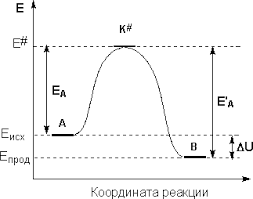
\includegraphics[width=\linewidth]{lecture_03/arrenius}
	\end{wrapfigure}
	\begin{gather*}
	K = \exp\left( -\dfrac{\Delta G^0}{kT} \right) \\
	E = E (\Delta G^0) = ?
	\end{gather*}
	
	Р.Маркус рассматривал реакции вида:
	\begin{gather*}
		A + D \xrightarrow{\hbar \omega} A^{-} + D^{+}
	\end{gather*}
	что представляет из себя переход $ e^{-} $ из $ D $ на $ A $.
	\begin{gather}
		\Delta G^0 = E_{D/D^{+}} - E_{A/A^{-}} - \hbar \omega - \dfrac{e^2}{\varepsilon a}
	\end{gather}

	\begin{figure}[H]
		\begin{minipage}[h]{0.26\linewidth}
			\centering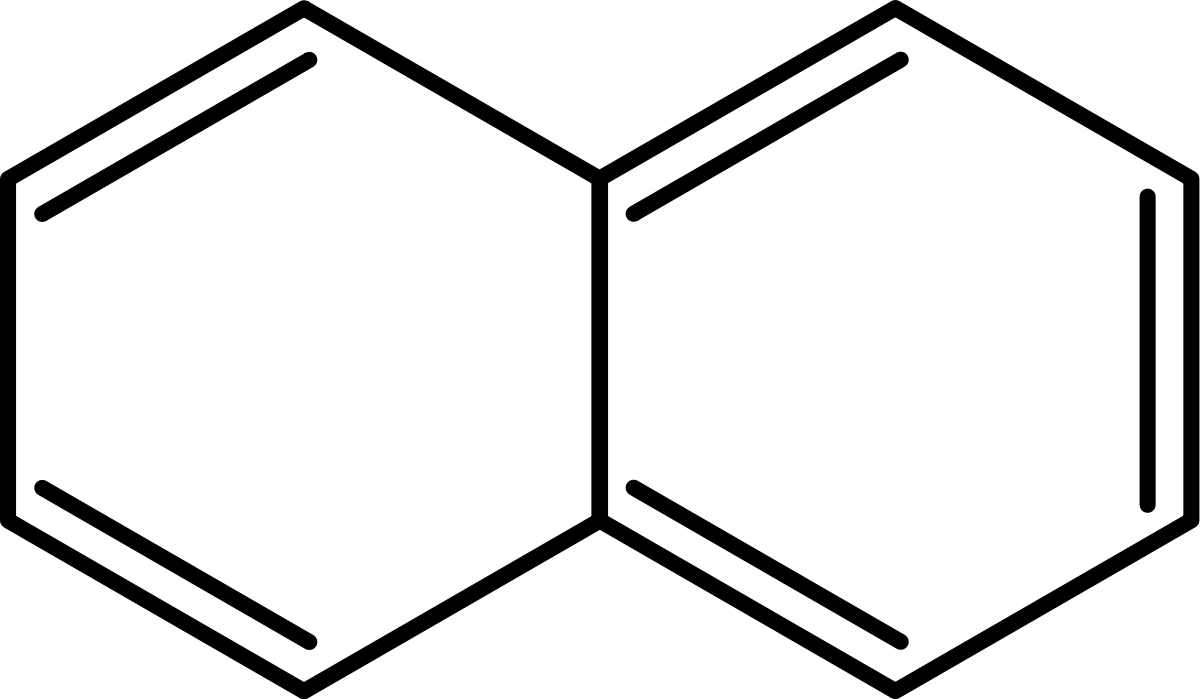
\includegraphics[width=\linewidth]{lecture_03/naftalin}
			\caption{Нафталин}
		\end{minipage}
		\hfill
		\begin{minipage}[h]{0.30\linewidth}
			\centering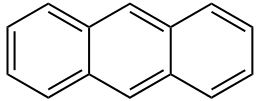
\includegraphics[width=\linewidth]{lecture_03/antracen}
			\caption{Антрацен}
		\end{minipage}
		\hfill
		\begin{minipage}[h]{0.28\linewidth}
			\centering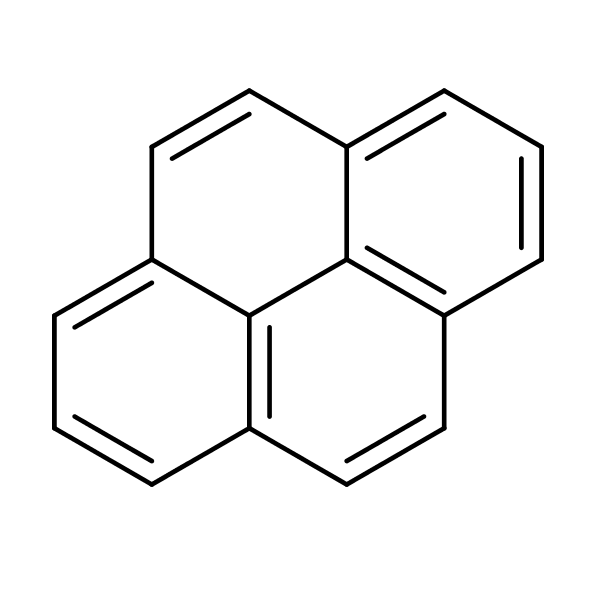
\includegraphics[width=\linewidth]{lecture_03/piren}
			\caption{Пирен}
		\end{minipage}
	\end{figure}

	\begin{wrapfigure}[12]{l}{0.45\linewidth}
%		\begin{tikzpicture}[line cap=round,line join=round,>=triangle 45,x=1.0cm,y=1.0cm]
%			\begin{axis}[
%				x=1.0cm,y=1.0cm,
%				axis lines=middle,
%				ymajorgrids=true,
%				xmajorgrids=true,
%				xmin=-7.0,
%				xmax=2.0,
%				ymin=-2.0,
%				ymax=6.0,
%				xtick={-7.0,-6.0,...,2.0},
%				ytick={-2.0,-1.0,...,6.0},
%				yticklabels={,,},
%				xticklabels={,,},
%				xlabel={$ \Delta G_0 $},
%				ylabel={$ \Delta G^{\neq} $}
%				]
%%				\clip(-7.,-2.) rectangle (2.,6.);
%				\draw [samples=50,rotate around={0.:(-3.,0.)},xshift=-3.cm,yshift=0.cm,line width=2.pt,domain=-8.0:8.0)] plot (\x,{(\x)^2/2/2.0});
%				\draw (-3.2427347858752804,0.6500525920360652) node[anchor=north west] {$-\lambda$};
%			\end{axis}
%		\end{tikzpicture}
		\centering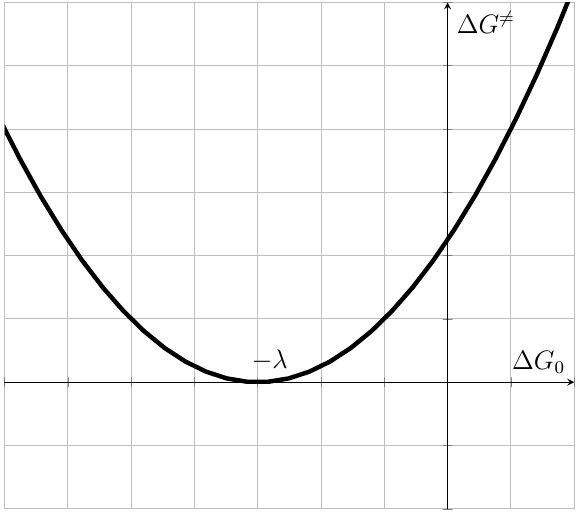
\includegraphics[width=\linewidth]{lecture_03/G_scheme}
		\caption{Схематическая зависимость $ \Delta G^{\neq} $}
	\end{wrapfigure}

	Считается, что энергию промежуточного комплекса можно представить выражением:
	\begin{gather*}
		\Delta G^{\neq} = \dfrac{(\lambda + \Delta G_0)^2}{4\lambda} \\
		\lambda \simeq 1 \text{ эВ (для полярных сред)}
	\end{gather*}

	Нужно помнить, что в равновесии 
	$ \Delta G = 0 $, но $ \Delta G_0 \neq 0 $.
%	Костыль, чтобы не наезжало на график
	\vspace{130pt}
		
	\end{lecSection}

	\begin{lecSection}[Электролитическая диссоциация]
		Электролитической диссоциации подвергаются вещества, которые полностью или частично состоят из ионов в растворе/расплаве.
		Вводится величина $ \alpha $ -- степень диссоциации (доля распавшихся на ионы молекул).
		Если $ \alpha \simeq 1 $, то вещество называется \textit{сильным электролитом}.
		
		Электролиты принято делить на \textbf{ионофоры} и \textbf{ионогены}. В \textit{ионофорах} ионы существуют до растворения. Пример: $ NaCl $. В \textit{ионогенах} -- наоборот. Пример: $ HCl $, для него диссоциация выглядит следующим образом:
		\begin{equation}
			HCl + H_2O \rightarrow \underbrace{H_3 O^{+}}_{\text{гидроксоний}} + Cl^{-}
			\label{chem:HCl_dissociation}
		\end{equation}
	\end{lecSection}
	% Исправление последствий костыля с \vspace выше
	\vspace*{-5cm}
\end{lecture}
